\documentclass{beamer}

\def\draft{draft}
\def\final{final}
\def\status{draft}
% !TeX root = ../thesis_presentation.tex
\usepackage[utf8]{inputenc}
\usepackage[T1]{fontenc}
\usepackage{lmodern}
\usepackage{times}
\usepackage[american]{babel}
\usepackage{tikz}
\usepackage{listings}
\usepackage{subcaption}
\usepackage{bm}
\usepackage{booktabs}
\usepackage{amsfonts}
\usepackage{amsmath}
\usepackage{amssymb}
\usepackage{amsthm}
\usepackage{marvosym}
\let\marvosymLightning\Lightning


%	Settings
%======================================================================
%%Tikz
\usetikzlibrary{shapes,arrows,calc,positioning,fit}

%% THEME: UOS-red or UOS-yellow
\usetheme{UOS}
% \usetheme[uosyellow]{UOS}

%% where to find the graphics
\graphicspath{{img/}}

%% Command setup
\newcommand{\source}[1]{\caption*{\textcolor{uos-grey-full}{Source: {#1}}} }
\newcommand{\RM}[1]{\MakeUppercase{\romannumeral{} #1{}}}
\newcommand{\code}[1]{\texttt{#1}}
\newcommand{\bull}[0]{\textbullet{}}
\newcommand{\tabitem}{{\color{uos-red-full}$\blacksquare$}}

% ---------------------------------------------------------------------
%% insert outline at begin of every section
\AtBeginSection[]{
  \frame{
    \frametitle{\iflanguage{ngerman}{Gliederung}{Outline}}
    \tableofcontents[current, currentsubsection]
  }
}

%% format: \title[short title]{long title}
%%   - short title will be used in foot line
%%   - long title will be used on title page
\title[Development with DevContainers]{Analysis of Adopting DevOps Tools for a Homogeneous Production and Development Environment}

% Color
\definecolor{codebg}{HTML}{EEEEEE}
\definecolor{dkgreen}{rgb}{0,0.6,0}
\definecolor{gray}{rgb}{0.5,0.5,0.5}
\definecolor{mauve}{rgb}{0.58,0,0.82}
\definecolor{LightCyan}{rgb}{0.88,1,1}



%======================================================================
% * * * * * * *   T E X T    S T A R T S    H E R E   * * * * * * * * *
%======================================================================
\begin{document}

\begin{frame}[plain]
  \titlepage{}
\end{frame}

\begin{frame}[allowframebreaks]{\iflanguage{ngerman}{Inhaltsverzeichnis}{Table of Contents}}
  \tableofcontents
\end{frame}

%%%%%%%%%%%%%%%%%%%%%%%%%%%%%%%%%%%%%%%%%%%%%%%%%%%%%%%%%%%%%%%%%%%%%%%%%%%%%%%%
% NOTES:
%%%%%%%%%%%%%%%%%%%%%%%%%%%%%%%%%%%%%%%%%%%%%%%%%%%%%%%%%%%%%%%%%%%%%%%%%%%%%%%%
\section{Goal of the Thesis}
\begin{frame}{Goal of the Thesis}
  \begin{itemize}
    \large
    \setlength\itemsep{1em}
    \setlength{\parskip}{12pt}
    \item Possibilities to increase efficiency in programming
          \begin{itemize}
            \large
            \setlength\itemsep{1em}
            \item Investigate possible points of improvement
            \item Developing an abstract solution concept
            \item Applying the concept to a prototype
            \item Evaluate and compare the concept to alternative solution
          \end{itemize}
  \end{itemize}
  \vfill
\end{frame}


%%%%%%%%%%%%%%%%%%%%%%%%%%%%%%%%%%%%%%%%%%%%%%%%%%%%%%%%%%%%%%%%%%%%%%%%%%%%%%%%
% NOTES:
% Studie von 2019 by ActiveState (Firma die sich auf coaching und Optimierung von Softwareprozessen spezialisiert)
% Habe mir dabei angesehen wie viele Stunden Entwickler nicht aktive coden
% Abseits von Software design und meeting Zeit sind dies die Tätigkeiten die am
% meisten Zeit in Anspruch nehmen.
% Neben Software Design und Meetings gehört auch Bug fixing dazu, dies hat aber
% Überschneidungen mit coding als auch mit Problemen in Konfigurationen und Dependencies
%%%%%%%%%%%%%%%%%%%%%%%%%%%%%%%%%%%%%%%%%%%%%%%%%%%%%%%%%%%%%%%%%%%%%%%%%%%%%%%%
\section{Problem Analyse}
\begin{frame}{}
  \begin{center}
    Potential Bottlenecks in the development workflow
    \vspace{0.5cm}
    \begin{columns}[totalwidth=\textwidth]
      \begin{column}{0.4\textwidth}
        \begin{itemize}
          \item Setup Configuration
          \item Testing
        \end{itemize}
      \end{column}
      \begin{column}{0.4\textwidth}
        \begin{itemize}
          \item Configuration
          \item Dependencies
        \end{itemize}
      \end{column}
    \end{columns}
  \end{center}
  \begin{figure}
    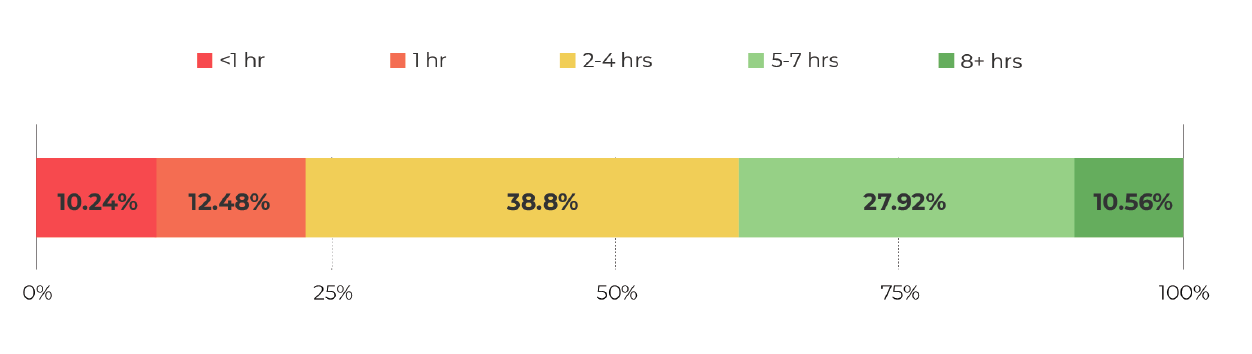
\includegraphics[width=0.8\textwidth]{coding_timepng.png}
    \caption{\footnotesize Hours spent programming \\\textcolor{uos-grey-full}{Source: {\cite{setuppain}}}}
  \end{figure}
\end{frame}

%%%%%%%%%%%%%%%%%%%%%%%%%%%%%%%%%%%%%%%%%%%%%%%%%%%%%%%%%%%%%%%%%%%%%%%%%%%%%%%%
% NOTES:
% Die Studie zeigt das die meisten Entwickler 1-4 mal im Jahr ihr System
% wechseln oder erneuern. Einige sogar deutlich öfter

% Dazu kommen neue Entwickler.
% Dies dauert bei den meisten 2-4 Stunden und bei 1/5 sogar zwischen 4 und 18 Stunden
% Für den GitHub.com Dienst haben die Entwickler ein scripts-to-rule-them-all geschrieben
% Dies dauerte allein 45 min für DB updates, oder dem installieren neuer dependencies beim wechseln von branches.
% Initiale Aufgaben wie E-Mail, VPN, Login für Git Lab/Hub, Jira etc. werden dabei nicht berücksichtigt
%%%%%%%%%%%%%%%%%%%%%%%%%%%%%%%%%%%%%%%%%%%%%%%%%%%%%%%%%%%%%%%%%%%%%%%%%%%%%%%%
\begin{frame}{}
  \begin{center}
    \Large Initial Setup
  \end{center}

  \begin{block}{}
    \begin{itemize}
      \small
      \setlength\itemsep{0em}
      \item 69\% of Developers renew their setup between 1-4 times a year
      \item 18\% even 5-8 times a year
    \end{itemize}
  \end{block}

  \begin{block}{}
    \begin{itemize}
      \small
      \setlength\itemsep{0em}
      \item 44\% of Developers need 2-4 hours to setup their Environment
      \item 14\% 4-8 hours and 6\% even over 18 hours
    \end{itemize}
  \end{block}

  \begin{block}{}
    \begin{itemize}
      \small
      \setlength\itemsep{0em}
      \item Installing development tools, language frameworks and IDEs
      \item Logging into E-Mail, VPN, messenger and network-shares
    \end{itemize}
  \end{block}
\end{frame}

%%%%%%%%%%%%%%%%%%%%%%%%%%%%%%%%%%%%%%%%%%%%%%%%%%%%%%%%%%%%%%%%%%%%%%%%%%%%%%%%
% NOTES:
% Und am Ende hat man das:
% Es fehlt immer noch ein Programm, eine Bibliothek oder es wurde eine falsche
% Version installiert. Die bringt uns zum Configurations und Dependency management
%%%%%%%%%%%%%%%%%%%%%%%%%%%%%%%%%%%%%%%%%%%%%%%%%%%%%%%%%%%%%%%%%%%%%%%%%%%%%%%%
\begin{frame}{}
  \vspace{-1cm}
  \begin{center}
    \Large Intensive Setup
  \end{center}
  \begin{figure}
    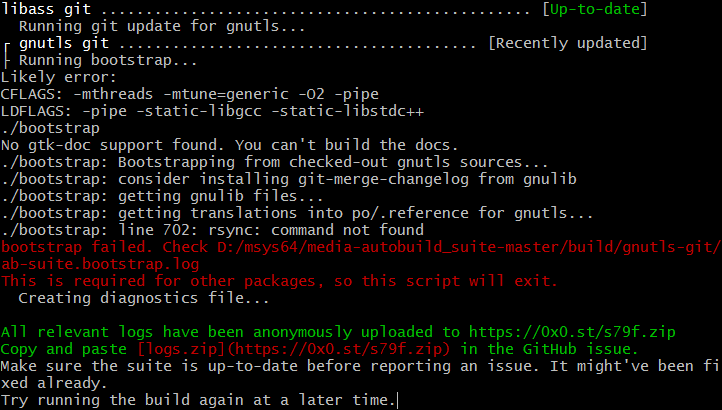
\includegraphics[width=0.8\textwidth]{img/terminal.png}
  \end{figure}
\end{frame}

%%%%%%%%%%%%%%%%%%%%%%%%%%%%%%%%%%%%%%%%%%%%%%%%%%%%%%%%%%%%%%%%%%%%%%%%%%%%%%%%
% NOTES:
% Das herstellen einer konsistenten und funktionierenden Entwicklungsumgebung
% über mehrere Entwickler (eventuell sogar verschiedene Betriebssysteme) ist eine
% enorme Herausforderung insbesondere in einer Microservice Architektur
% Man muss:
% Über Umgebungsvariablen werden in der regel Einstellungen wie HOST, PORT, USER und PW
% für Datenbanken und andere Einstellungen übergeben. Weiteres sind z.B. API Keys
% Die Komplexität nimmt exponential zu wenn man viele Anwendungen hat die auch noch untereinander Kommunizieren APP B -> zu APP A ...

% Oftmals gibt es dann auch noch unterschiede bei den Dependencies.
% Entwickler die an mehreren Projekten Arbeiten (häufig) müssen eventuelle
% NodJS 12 für ein Projekt und NodeJS 14 für ein anderes benutzen.
% Dazu kommen die zwischen Development und Production Umgebung.
% Production läuft oft Linux 75.3% aller Webserver (w3techs) & Development oft Windows 40% Linux 25% MacOs 25% StackOverflow 2021

% Einiges wird unter Windows auch nicht mehr unterstützt. Keine Entwicklung von Lagacy PHP unter Windows

%%%%%%%%%%%%%%%%%%%%%%%%%%%%%%%%%%%%%%%%%%%%%%%%%%%%%%%%%%%%%%%%%%%%%%%%%%%%%%%%
\begin{frame}{}
  \begin{center}
    \Large Configuration \& Dependencies
  \end{center}

  \begin{block}{}
    \begin{itemize}
      \small
      \setlength\itemsep{0em}
      \item APP A needs a DB connection string with: host, user, password
      \item APP B listens on port 8080 and requests APP A on port 3000
    \end{itemize}
  \end{block}
  \begin{block}{}
    \begin{itemize}
      \small
      \setlength\itemsep{0em}
      \item Project A requires NodeJS V12 \text{\marvosymLightning} Project B requires NodeJS V14
      \item Development uses Python 3.9 \text{\marvosymLightning} Production uses Python 3.7
      \item Development uses PHP 7.3 \text{\marvosymLightning} Production uses legacy PHP \(\leq 7.0\)
    \end{itemize}
  \end{block}
\end{frame}

%%%%%%%%%%%%%%%%%%%%%%%%%%%%%%%%%%%%%%%%%%%%%%%%%%%%%%%%%%%%%%%%%%%%%%%%%%%%%%%%
% NOTES:
% Das sind nur die Runtime Dependencies - Dependencies zwischen Anwendungen können zur
% enormen Herausforderung werden. Alle einzelnen Anwendung müssen gestartet und dessen output überwacht werden

% Das sind alle Services die XXX bei Netflix liefen. Die wird NICHT alle lokal laufen lassen
% Aber allein ein Bruchteil davon auf dem lokalen auf dem PC zu installieren und zu starten kann schnell unübersichtlich und Fehleranfällig werden
%%%%%%%%%%%%%%%%%%%%%%%%%%%%%%%%%%%%%%%%%%%%%%%%%%%%%%%%%%%%%%%%%%%%%%%%%%%%%%%%
\begin{frame}{}
  \begin{center}
    \Large Configuration \& Dependencies
  \end{center}
  \begin{figure}
    %  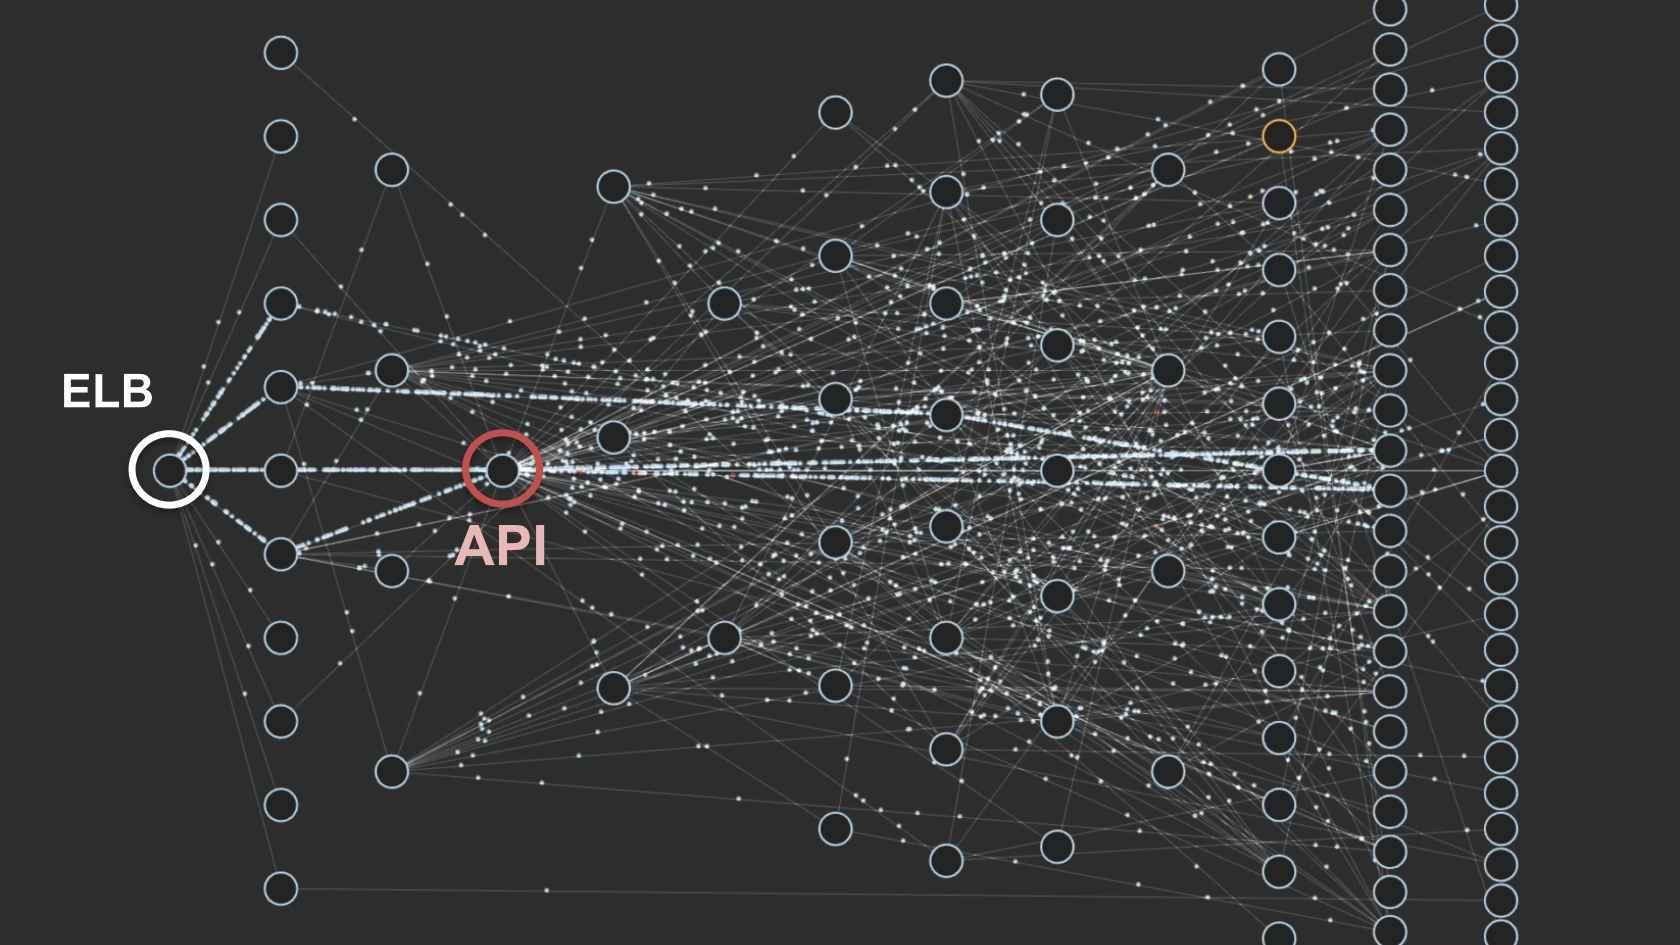
\includegraphics[width=0.8\textwidth]{img/netflix.jpg}
    % \caption{Netflix Microservice Graph}
    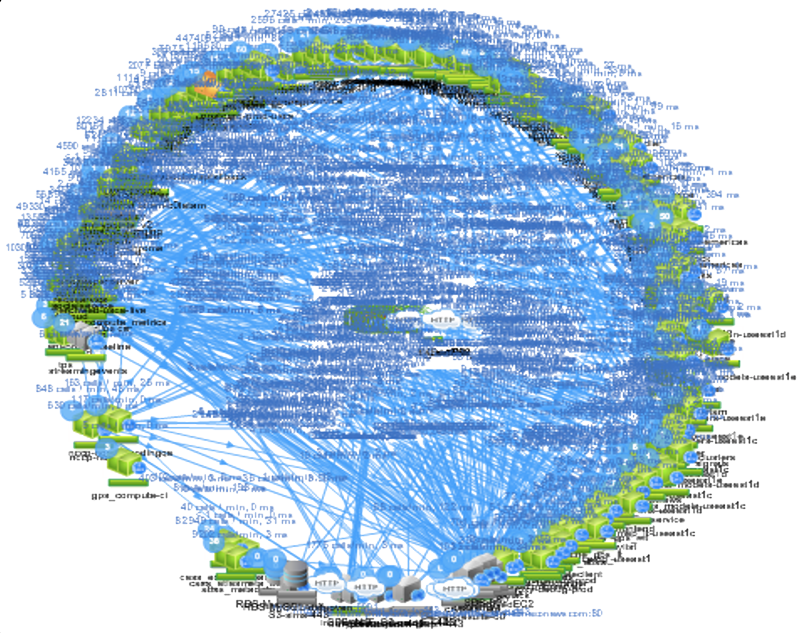
\includegraphics[width=0.6\textwidth]{img/netfix.png}
    \caption{\footnotesize Netflix's Microservice Death-Star \\\textcolor{uos-grey-full}{Source: {\cite{deathstar}}}}
  \end{figure}
\end{frame}

%%%%%%%%%%%%%%%%%%%%%%%%%%%%%%%%%%%%%%%%%%%%%%%%%%%%%%%%%%%%%%%%%%%%%%%%%%%%%%%%
% NOTES:
% Wenn man ein Service Mesh hat dann ist Testing eine große Herausforderung, auch bei kleineren Diensten
% Wenn man sich die Testing Pyramide wieder in Erinnerung ruft dann kann man quasi nur noch die Unit tests ausführen bevor man seine Änderungen in VCS pusht
% Alles andere wird zu aufwendig auf dem lokalen PC zu installieren.
% Zwar gibt es Mock Server, und API validations zum testen, diese garantieren jedoch nicht dass zwei Services wirklich erfolgreich kommunizieren können.
% Deswegen können in einer MSA viele tests nur in der CI ausgeführt werden. Dort dauert es viel länger bis ein Fehler gefunden wird und das verlangsamt und verteuert den Entwicklungsprozess
%%%%%%%%%%%%%%%%%%%%%%%%%%%%%%%%%%%%%%%%%%%%%%%%%%%%%%%%%%%%%%%%%%%%%%%%%%%%%%%%
\begin{frame}{}
  \vspace{-0.5cm}
  \begin{center}
    \Large Testing
  \end{center}

  \vspace{-0.5cm}
  \begin{figure}
    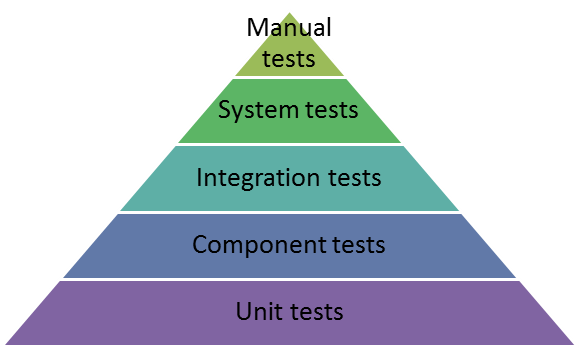
\includegraphics[width=0.58\textwidth]{img/tests-pyramid.png}
    \caption{\footnotesize The Test-Pyramid - \textcolor{uos-grey-full}{Source: {\cite{microtest}}}}
  \end{figure}
  \vspace{-0.2cm}
  \begin{block}{}
    \begin{itemize}
      \small
      \setlength\itemsep{0em}
      \item Increased testing effort in a Microservice architecture
      \item Late error detection \(\Rightarrow \) higher repair time and costs
    \end{itemize}
  \end{block}
\end{frame}


\section{Concept \& Prototype}
%%%%%%%%%%%%%%%%%%%%%%%%%%%%%%%%%%%%%%%%%%%%%%%%%%%%%%%%%%%%%%%%%%%%%%%%%%%%%%%%
% NOTES:
%%%%%%%%%%%%%%%%%%%%%%%%%%%%%%%%%%%%%%%%%%%%%%%%%%%%%%%%%%%%%%%%%%%%%%%%%%%%%%%%
\begin{frame}{}
  \begin{center}
    \Large Apply solutions from the server world
  \end{center}
  \vspace{.8cm}
  \begin{itemize}
    \setlength\itemsep{1.2em}
    \large
    \item Abstracting the underlying hardware and system
    \item Define and standardize the working environments
    \item Reduce manual effort and automate processes
    \item Allow integration on the developer system
  \end{itemize}
\end{frame}

\begin{frame}{}
  \begin{columns}[totalwidth=\textwidth]
    \begin{column}{0.5\textwidth}
      \begin{figure}
        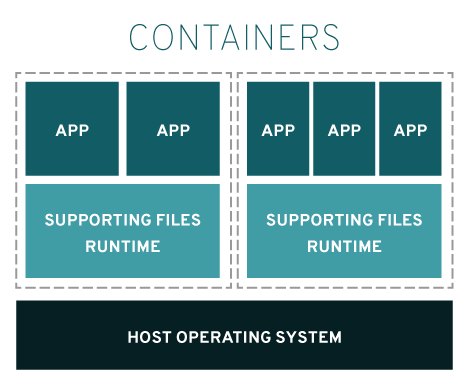
\includegraphics[width=1.1\textwidth]{img/docker-vm-redhat.png}
        \caption{\footnotesize Container based virtualization - \textcolor{uos-grey-full}{Source: {\cite{redhat_pic}}}}
      \end{figure}
    \end{column}
    \begin{column}{0.4\textwidth}
      \begin{itemize}
    \setlength\itemsep{0.6em}
        \item Container based virtualization
        \item Lightweight as only processes are isolated
        \item The app runtime is in a self-contained bundle
        \item Implemented with Docker
      \end{itemize}
    \end{column}
  \end{columns}
\end{frame}



\section{Evaluation}
%%%%%%%%%%%%%%%%%%%%%%%%%%%%%%%%%%%%%%%%%%%%%%%%%%%%%%%%%%%%%%%%%%%%%%%%%%%%%%%%
% NOTES:
%%%%%%%%%%%%%%%%%%%%%%%%%%%%%%%%%%%%%%%%%%%%%%%%%%%%%%%%%%%%%%%%%%%%%%%%%%%%%%%%
\begin{frame}{Data analysis}
  \vspace{-0.2cm}
  \begin{columns}[totalwidth=\textwidth]
    \begin{column}{\textwidth}
      \begin{table}
        \scalebox{0.7}{
          \begin{tabular}{@{}l|l|l|l|l|l|l@{}}
            \toprule
            Number of subflows        & 1       & 2       & 3      & 4      & 5      & \textgreater{}5 \\ \midrule\midrule
            Percentage of connections & 67.75\% & 29.96\% & 1.07\% & 0.48\% & 0.26\% & 0.48\%          \\ \bottomrule
          \end{tabular}
        }
        \caption{\footnotesize Number of subflows per MPTCP connection, \textcolor{uos-grey-full}{Source:\cite{realMPTCP}}}
      \end{table}
    \end{column}
  \end{columns}

  \ifx\status\final{}
    \pause{}
  \fi

  \vspace{-0.5cm}
  \begin{table}[]
    \scalebox{0.7}{
      \begin{tabular}{@{}l|l|l|l|l@{}}
        \toprule
        \textbf{Port} & \textbf{\# connections} & \textbf{\% connections} & \textbf{Bytes} & \textbf{\% bytes} \\ \midrule\midrule
        53            & 107,012                 & 27.4                    & 17.4 MB        & \textless{}0.1    \\ \midrule
        80            & 103,597                 & 26.5                    & 14,943 MB      & 58.8              \\ \midrule
        443           & 104,223                 & 26.7                    & 9,253 MB       & 36.4              \\ \midrule
        4070          & 571                     & 0.1                     & 91.7 MB        & 0.4               \\ \midrule
        5228          & 10,602                  & 2.7                     & 27.3           & 0.1               \\ \midrule
        8009          & 10,765                  & 2.8                     & 0.97           & \textless{}0.1    \\ \midrule
        Others        & 54,012                  & 13.8                    & 1.090 MB       & 4.4               \\ \bottomrule
      \end{tabular}\label{tab:traffic}
    }
    \caption{\footnotesize Statistics about destination port, \textcolor{uos-grey-full}{Source:~\cite{realMPTCP}}}
  \end{table}

  %\textcolor{uos-red-full}{\Large{\(\bm{\Rightarrow}\)}} Won't result in ONE good application
\end{frame}



%%%%%%%%%%%%%%%%%%%%%%%%%%%%%%%%%%%%%%%%%%%%%%%%%%%%%%%%%%%%%%%%%%%%%%%%%%%%%%%%
% Netzwerke sind unterschiedlich
% RTT, Bandbreite, Zuverlässigkeit
%%%%%%%%%%%%%%%%%%%%%%%%%%%%%%%%%%%%%%%%%%%%%%%%%%%%%%%%%%%%%%%%%%%%%%%%%%%%%%%%
\begin{frame}{Asymmetric paths}

  \begin{center}
    \Large \color{uos-red-full} Multiple subflows have different characteristics in terms of:
  \end{center}
  \vspace{0.5cm}

  %\pause

  \begin{table}
    \centering
    \begin{tabular}{@{}l@{}}
      \large\tabitem{} Round Trip Time (Latency) \\[10pt]
      \large\tabitem{} Bandwidth (Throughput)    \\[10pt]
      \large\tabitem{} Error rate (Reliability)
    \end{tabular}
  \end{table}
\end{frame}


\begin{frame}{Lowest-RTT-First}
  \begin{columns}
    \begin{column}{0.48\textwidth}
      \begin{enumerate}
        \setlength\itemsep{1.2em}
        \item Uses the subflow with the lowest RTT
              \setcounter{enumi}{2}
        \item Use next lowest RTT
      \end{enumerate}
    \end{column}

    \begin{column}{0.48\textwidth}
      \begin{enumerate}
        \setlength\itemsep{1.2em}
        \setcounter{enumi}{1}
        \item Until congestion window is filled
              \setcounter{enumi}{3}
        \item Standard Linux scheduler
      \end{enumerate}
    \end{column}
  \end{columns}

  \vspace{0.8cm}
  {\color{uos-red-full}\rule{\textwidth}{1.5pt}}
  %\pause

  \begin{table}[]
    \begin{tabular}{@{}lll@{}}
      \(err\)             & \(=\) & \(measured_{RTT} - predic\)                               \\
      \(predic_{new}\)    & \(=\) & \(predic_{old} + \frac{1}{8} * err\)                      \\
      \(variation_{new}\) & \(=\) & \(\frac{3}{4} * variation_{old} + \frac{1}{4} * \|err\|\) \\
      \(RTO\)             & \(=\) & \(predic + 4 * variation\)
    \end{tabular}
    \caption{\small Jacobson’s Algorithm}
  \end{table}
\end{frame}


\begin{frame}{Performance baseline}
  \begin{columns}
    \vspace{-2cm}
    \begin{column}{0.38\textwidth}
      \small
      \bull{} Results for LRF, DAPS, OTIAS, ECF\\
      \vspace{0.3cm}
      \bull{} Figure a): WLAN/3G setup \\
      \vspace{0.3cm}
      \bull{} Figure b): WLAN/WLAN setup\\
      \vspace{0.3cm}
      \bull{} All schedulers perform similarly with marginal differences in a)\\
      \vspace{0.3cm}
      \bull{} Increased page load times for DAPS and OTIAS in b)\\
    \end{column}
    \begin{column}{0.58\textwidth}
      \vspace{-0.8cm}
      \begin{figure}
        \centering
        % \includegraphics[width=0.90\textwidth]{default_sched_base.jpg}\label{fig::base}
        \vspace{-0.2cm}
        \caption{\footnotesize Page load time for web traffic, \textcolor{uos-grey-full}{Source: {\cite{lowlatschedulers}}}}
      \end{figure}
    \end{column}
  \end{columns}
\end{frame}


\appendix
\begin{frame}[allowframebreaks]{References}
  \small
  \setbeamertemplate{bibliography item}[book]
  \bibliography{bib/mybib}{}
  \bibliographystyle{IEEEtranSA}
\end{frame}

\begin{frame}{Questions?}
  \begin{center}
    Thank you for your attention!

    Any questions?
  \end{center}
\end{frame}


\begin{frame}[fragile]{Shortest Transfer Time First}
  \begin{lstlisting}[frame=single, basicstyle=\tiny, caption={STTF pseudo code,  \textcolor{uos-grey-full}{Source: \cite{lowlatschedulers}}}, label=code::sttf]
  function TRANSFER_TIME:
      if cwnd_free > 0 and data_to_send < cwnd_free then
          return rtt / 2
      transfer_time = transfer_time + rtt
      cwnd = increase_cwnd(current_cc_state)

      if data_to_send <= max_segments_in_ss then
          transfer_time = transfer_time + rtt * (rounds_in_ss-1) + rtt/2
          return transfer_time
      else if cwnd < ssthresh then
          transfer_time = transfer_time + max_rounds_in_ss * rtt
      if ends_in_ss(data_to_send) then
          return transfer_time

      cwnd = ssthresh
      transmission_time += rtt * (rounds_in_ca - 1) + rtt / 2
    return transfer_time
  \end{lstlisting}
\end{frame}

\end{document}
